\section{Properties of Probability measures}
Let $(\Omega, \mathcal{F}, \mathbb{P})$ be a probability space and $\mathbb{P} : \mathcal{F} \to [0, 1]$.

\begin{definition}[Countable additivity]
    P3 : $\mathbb{P}(\bigcup_{n \in \mathbb{N}} A_n) = \sum_{n \in \mathbb{N}} \mathbb{P}(A_n)$ for $(A_n)_{n \in \mathbb{N}}$ disjoint.
\end{definition} 

\begin{question}
    What if the sets are not disjoint?
\end{question} 

\subsection{Countable sub-additivity}

\begin{proposition}[Countable sub-additivity]
    Let $(A_n)_{n\geq 1}$ be a sequence of events in $\mathcal{F}$.
    Then
    \begin{align*}
        \mathbb{P}\left(\bigcup_{n \in \mathbb{N}} A_n\right) \leq \sum_{n \in \mathbb{N}} \mathbb{P}(A_n).
    \end{align*} 
\end{proposition} 

\emph{Intuition}:
\begin{figure}[h] 
    \centering 
    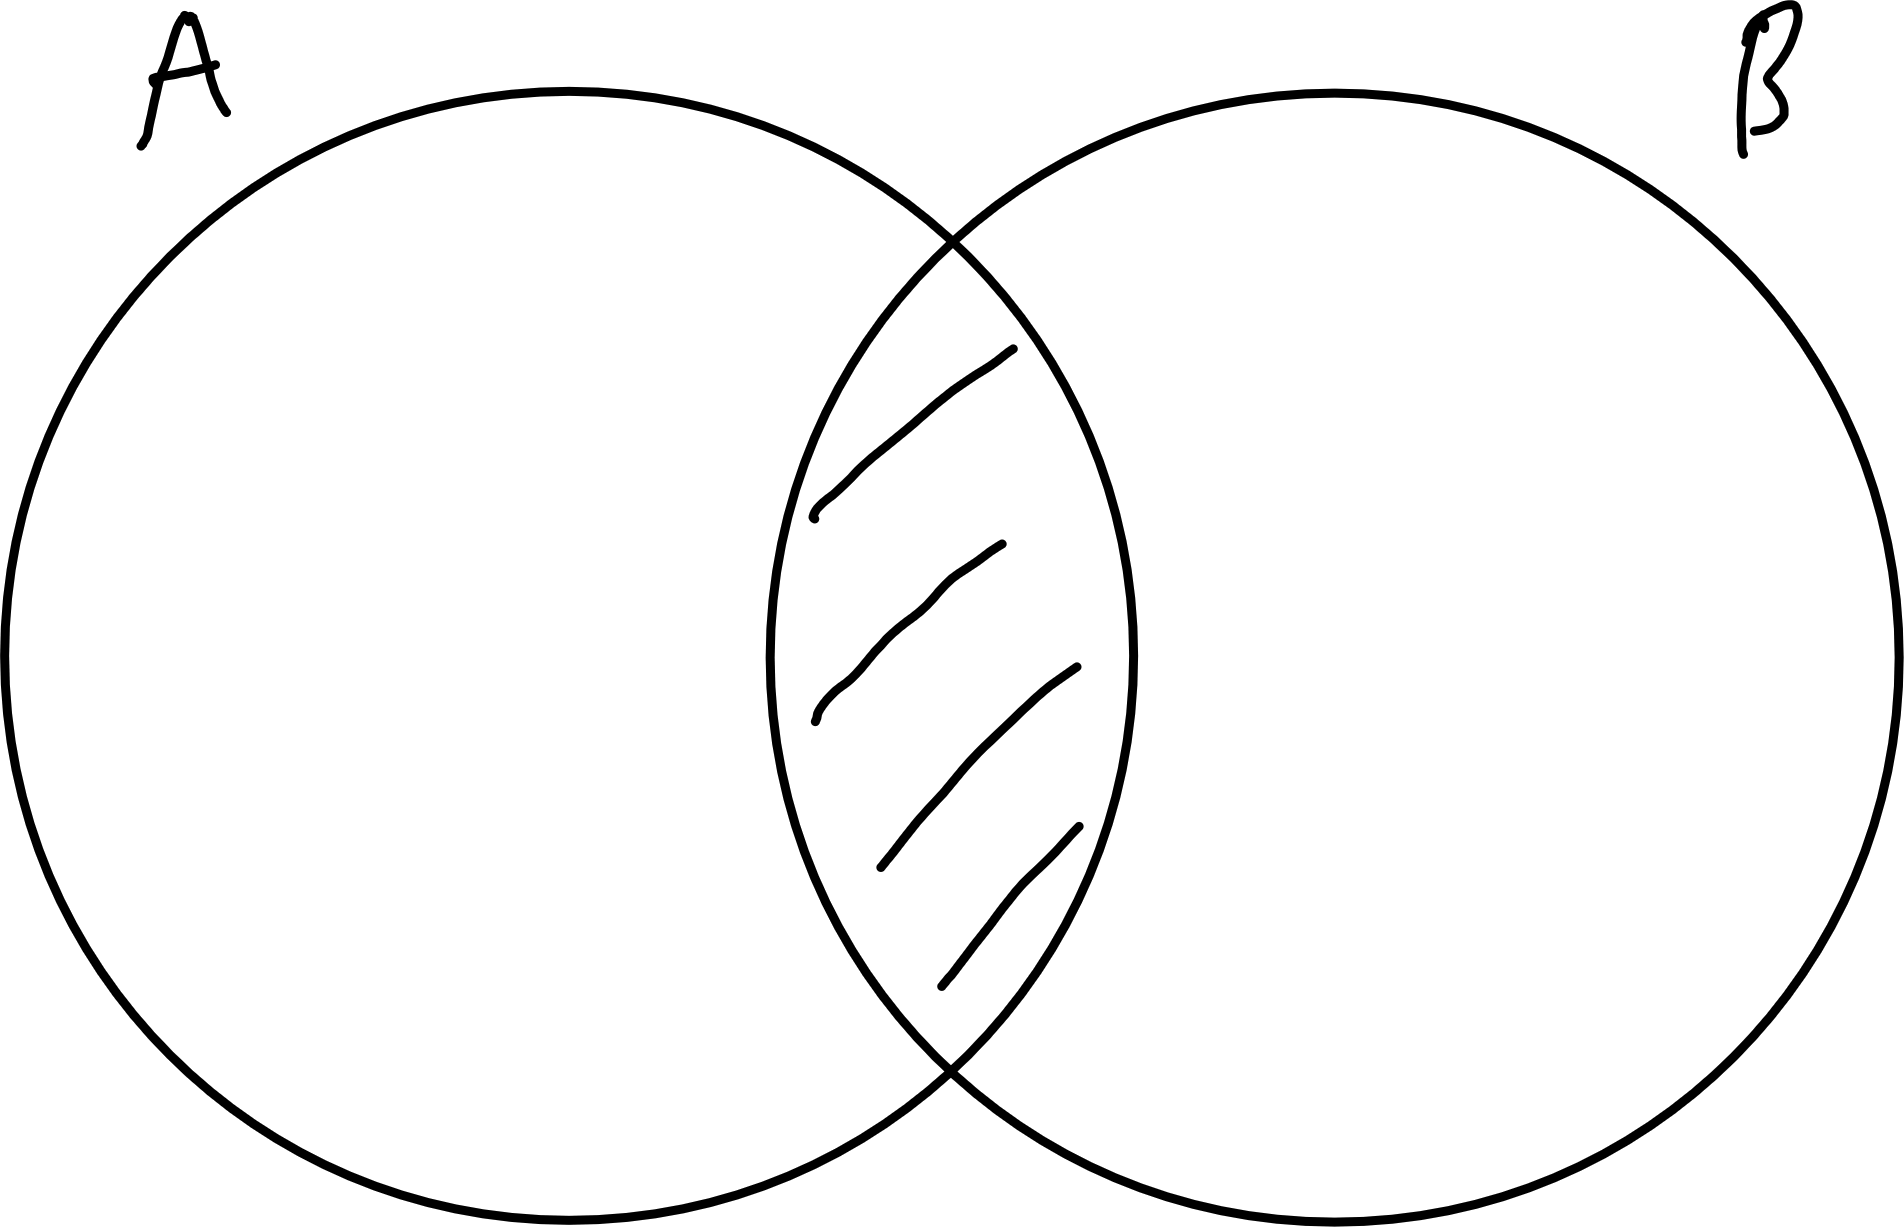
\includegraphics[height=5cm]{03-venn-diagram} 
\end{figure}

$\sum_{n \in \mathbb{N}} \mathbb{P}(A_n)$ ``double counts" some sub-events.

\begin{proof}
    \emph{Idea}: Rewrite $\bigcup_{n \in \mathbb{N}} A_n$ as a \emph{disjoint} union.
    Define $B_1 = A_1$ and $B_n = \underbracket{A_n \setminus (A_1\cup \dots \cup A_{n-1})}_{\in \mathcal{F} (\text{by Sheet 1})}\quad \forall \; n \geq 2$.
    {\par \centering 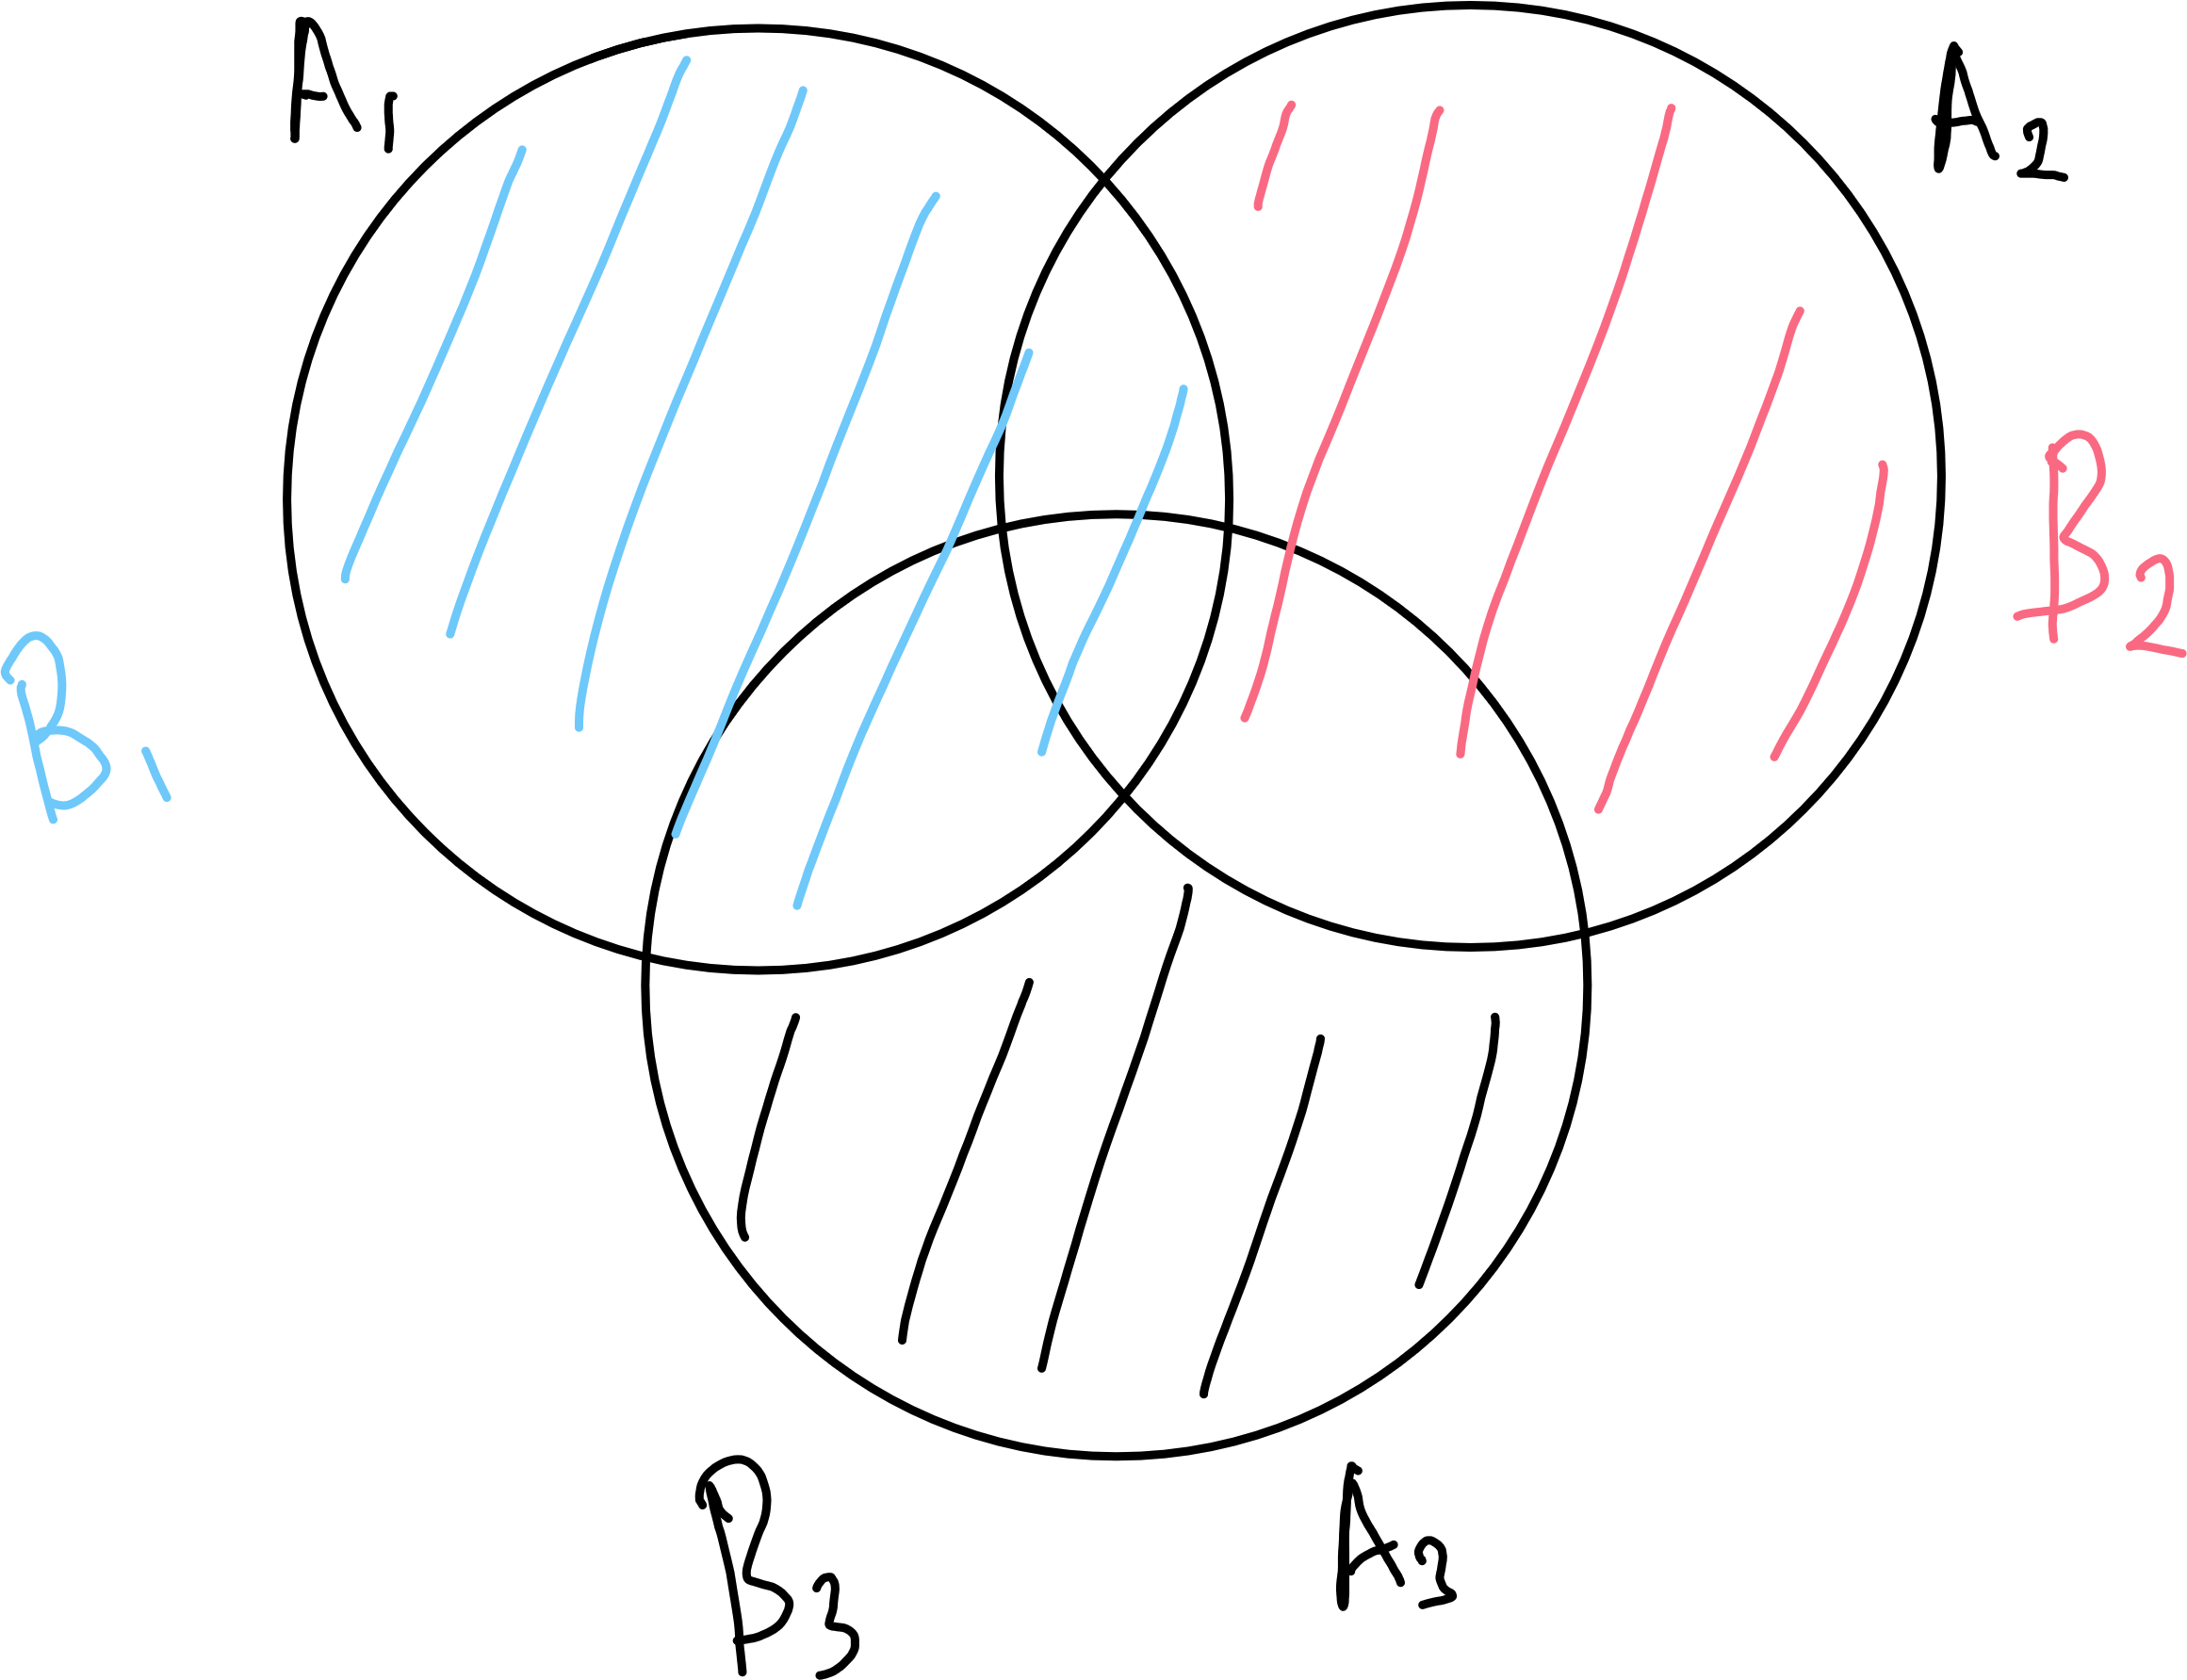
\includegraphics[height=5cm]{03-subadditivity} \par}
    So
    \begin{itemize}
        \item $\bigcup_{n \in \mathbb{N}} B_n = \bigcup_{n \in \mathbb{N}} A_n$.
        \item $(B_n)_{n \in \mathbb{N}}$ is disjoint (by construction).
        \item $B_n \subseteq A_n \implies \underbracket{\mathbb{P}(B_n) \leq \mathbb{P}(A_n)}_ {\text{Q4, Sheet 1}}$
    \end{itemize} 
    \begin{align*}
        \mathbb{P}\left(\bigcup_{n \in \mathbb{N}} A_n\right) = \mathbb{P}\left(\bigcup_{n \in \mathbb{N}} B_n\right) \underset{P3 \text{ on } (B_n)}{=} \sum_{n \in \mathbb{N}}  \mathbb{P}\left(B_n\right) \leq \sum_{n \in \mathbb{N}} \mathbb{P}\left(A_n\right)
    \end{align*} 
\end{proof} 

\subsection{Continuity}

\begin{proposition}[Continuity]
    Let $(A_n)_{n \in \mathbb{N}}$ be an increasing sequence of events in $\mathcal{F}$, i.e. $A_n \subseteq A_{n + 1} \quad \forall \; n$. 
    Then $\mathbb{P}(A_n) \leq \mathbb{P}(A_{n + 1})$.
    So $\mathbb{P}(A_n)$ converges as $n \to \infty$.\footnote{As probabilities are bounded above by 1 and increasing.}

    \emph{In fact:} $\lim_{n \to \infty} \mathbb{P}(A_n) = \mathbb{P} \left(\bigcup_{n \in \mathbb{N}} A_n \right)$.
\end{proposition} 

For motivation try Q6, Sheet 1.

\begin{figure}[h] 
    \centering 
    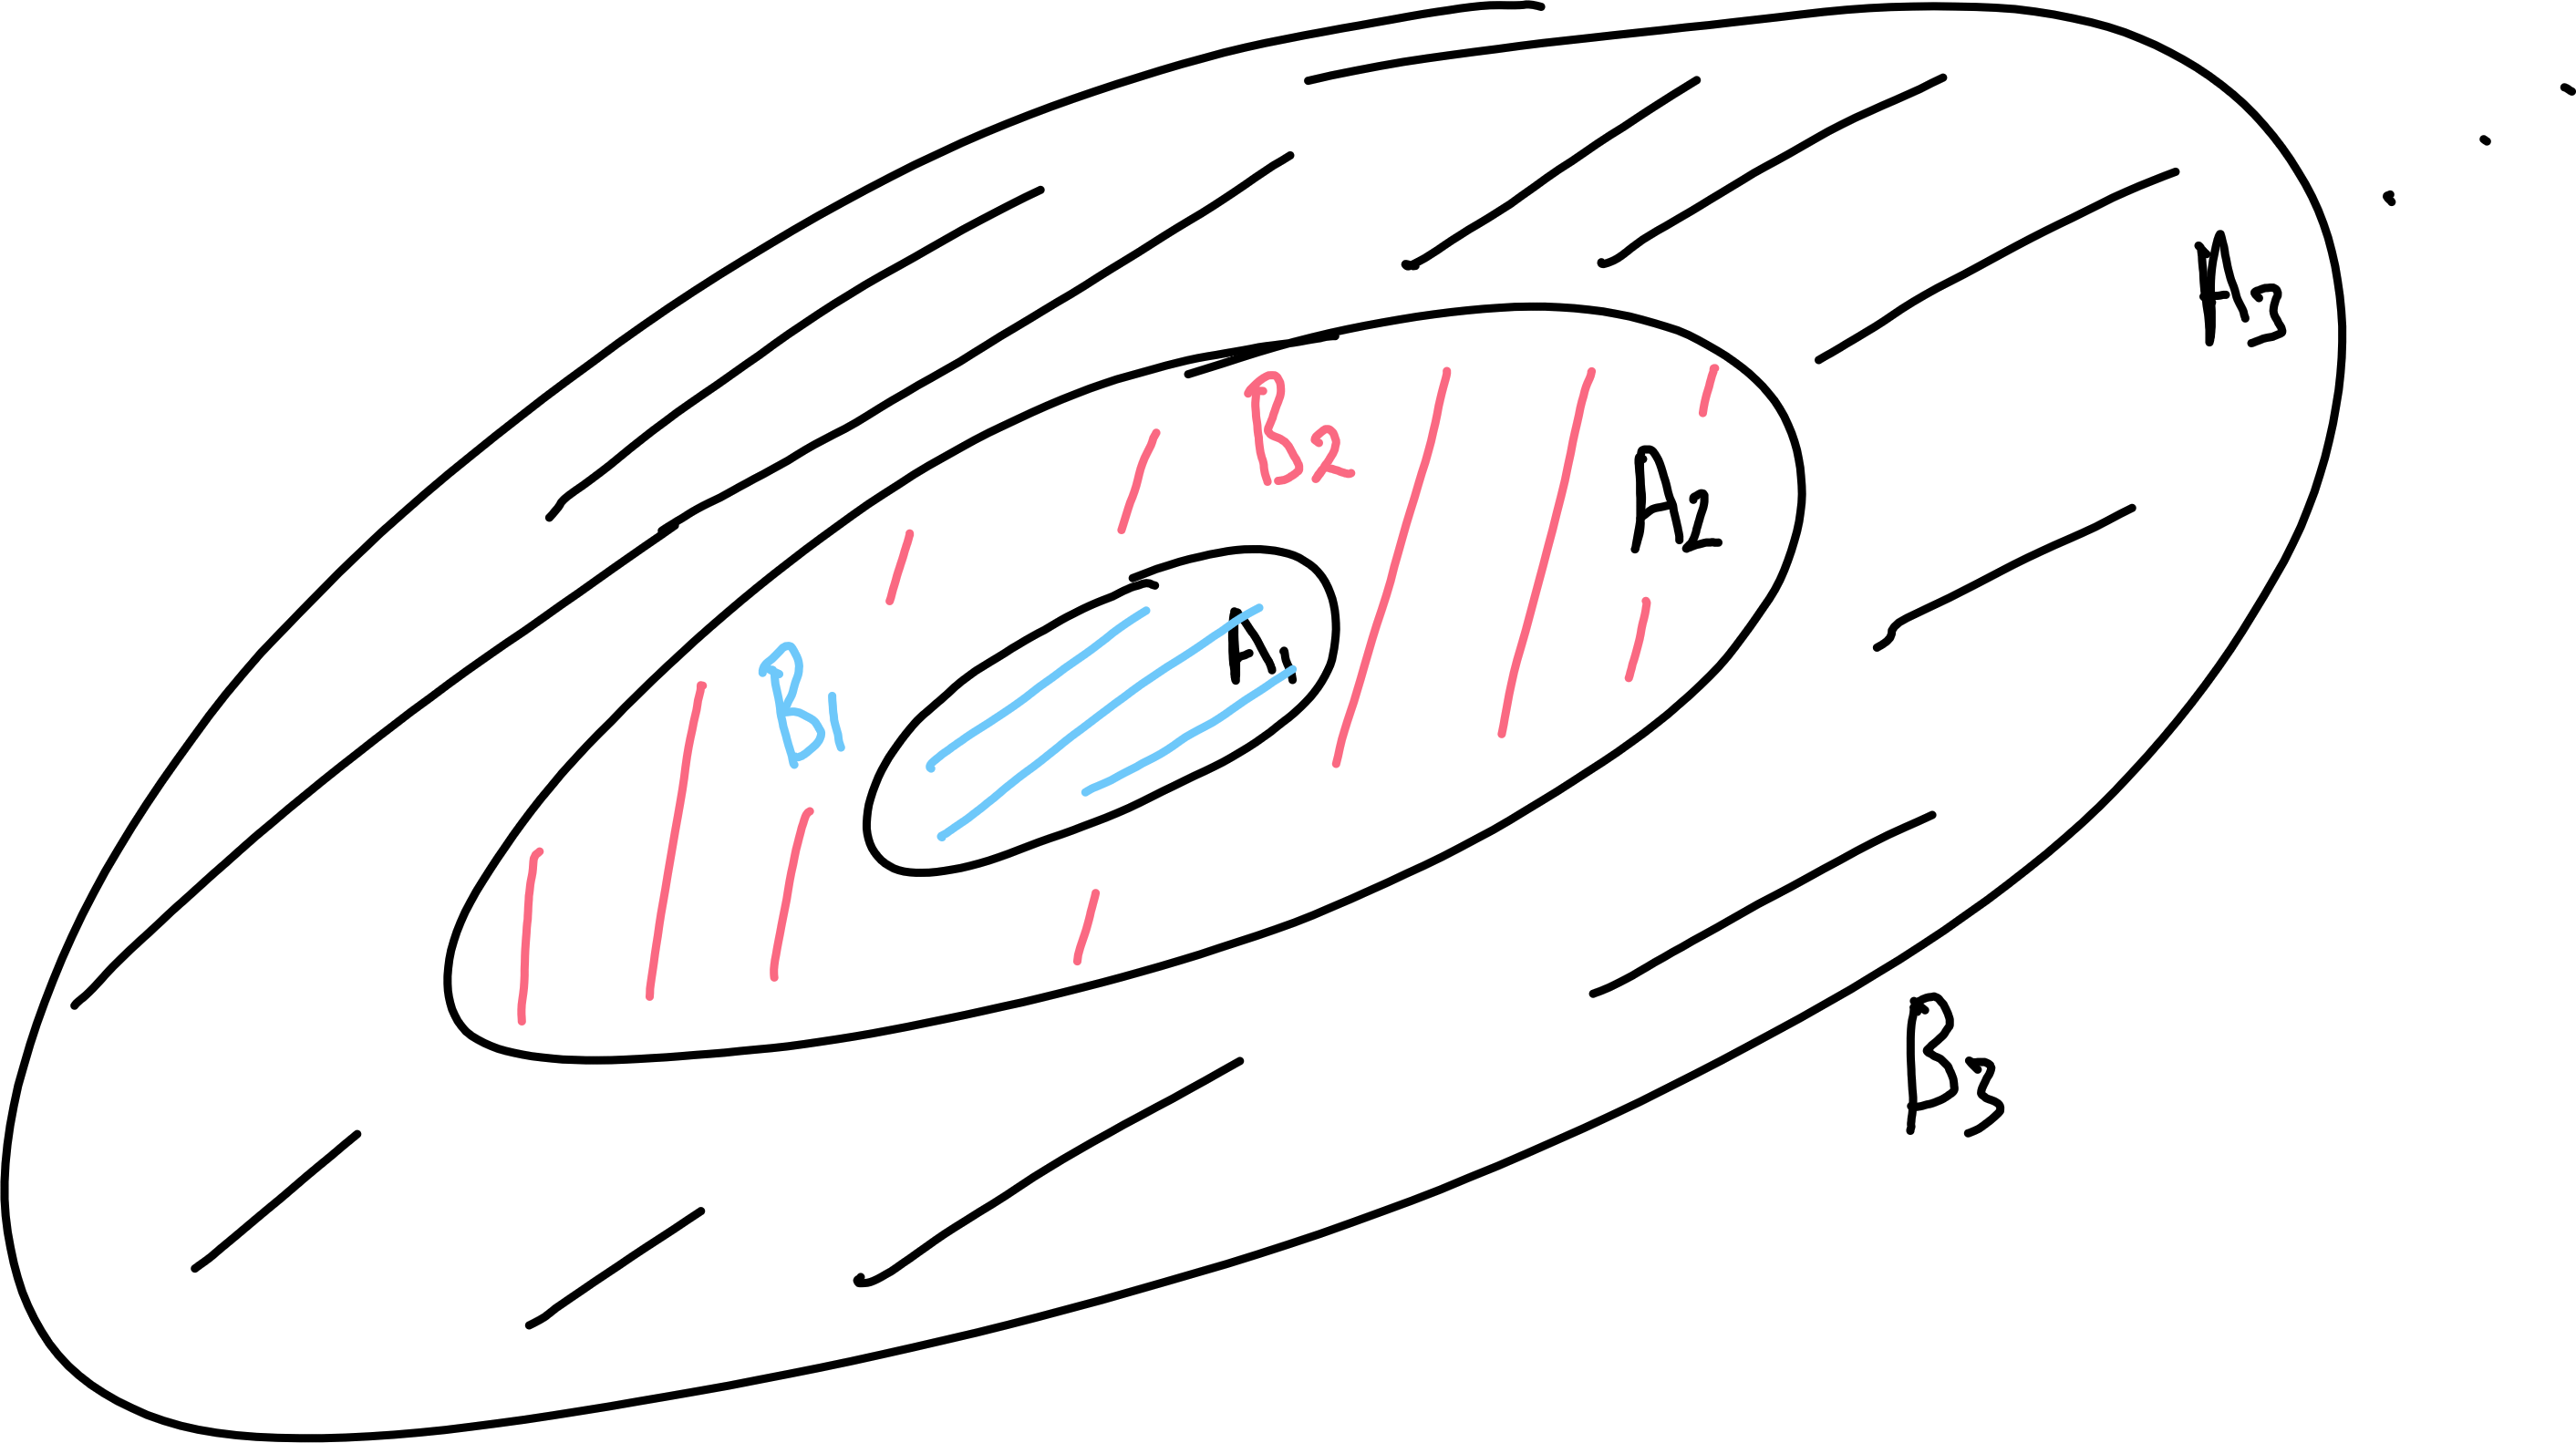
\includegraphics[height=5cm]{03-continuity} 
\end{figure}

\begin{proof}
    Let us reuse the $B_n$s from the previous subsection.
    \begin{itemize}
        \item $\bigcup_{k = 1}^n B_k = A_n$ (disjoint union).
        \item $\bigcup_{n \in \mathbb{N}} B_n = \bigcup_{n \in \mathbb{N}} A_n$
    \end{itemize} 
    \begin{align*}
        \mathbb{P}(A_n) &= \sum_{k=1}^{n} \mathbb{P}(B_k) \overset{n \to \infty}{\to} \sum_{k \geq 1} \mathbb{P}(B_k) = \mathbb{P} \left(\bigcup_{n \in \mathbb{N}} B_n \right) = \mathbb{P} \left(\bigcup_{n \in \mathbb{N}} A_n \right) 
    \end{align*} 
\end{proof} 

\subsection{Inclusion-Exclusion Principle}

Background: $\mathbb{P}(A \cup B) = \mathbb{P}(A) + \mathbb{P}(B) - \mathbb{P}(A \cup B)$. \\
Similarly: $A, B, C \in \mathcal{F}$
\begin{align*}
    \mathbb{P}(A \cup B \cup C) &= \mathbb{P}(A) + \mathbb{P}(B) + \mathbb{P}(C) - \mathbb{P}(A \cup B) - \mathbb{P}(B \cup C) - \mathbb{P}(C \cup A) + \mathbb{P}(A \cap B \cap C).
\end{align*} 

\begin{proposition}[Inclusion-Exclusion Principle]
    Let $A_1, \dots, A_n \in \mathcal{F}$, then:
    \begin{align*}
        \mathbb{P} \left(\bigcup_{i = 1}^n A_i \right) = &\sum_{i=1}^{n} \mathbb{P}(A_i) - \sum_{1 \leq i_1 < i_2 \leq n} \mathbb{P}(A_{i_1} \cap A_{i_2}) + \sum_{1 \leq i_1 < i_2 < i_3 \leq n} \mathbb{P}(A_{i_1} \cap A_{i_2} \cap A_{i_3}) - \dots \\ &+ (-1)^{n + 1} \mathbb{P}(A_1 \cap \dots \cap A_n) \\
        = &\sum_{\substack{I \subset \{1, \dots, n\} \\ I \neq \emptyset} } (-1)^{|I| + 1} \mathbb{P} \left( \bigcap_{i \in I} A_i \right)
    \end{align*}
    Note: $\sum_{1 \leq i_1 < i_2 \leq n}$ is the sum of all triples that are distinct and unordered.
\end{proposition}